\documentclass[11pt,a4paper]{article}

\usepackage[utf8]{inputenc}
\usepackage[T1]{fontenc}
\usepackage{lmodern}
\usepackage[margin=1in]{geometry}
\usepackage{amsmath,amssymb,amsfonts}
\usepackage{booktabs}
\usepackage{array}
\usepackage{graphicx}
\usepackage{float}
\usepackage{caption}
\usepackage{xcolor}
\usepackage[colorlinks=true,linkcolor=blue!70!black,urlcolor=blue!70!black,citecolor=blue!70!black]{hyperref}

% Automatically find figures whether uploaded in Overleaf root (./) or inside figures/
\graphicspath{{./}{figures/}{../figures/}{../../figures/}}

\setlength{\parskip}{0.4em}
\setlength{\parindent}{1.2em}

\title{\textbf{Statistical Foundations to Reproducible Research ---\\Phase 1 Report}\\
\large An Empirical Investigation of Body Mass Index, Systolic Blood Pressure, and\\
Demographic Structure in US Adults (NHANES 2021--2023)}

\author{Author: \textbf{Ali Nowzari} \quad --- \quad Student ID: \textbf{403100292}\\
Track A: CDC/NCHS National Health and Nutrition Examination Survey\\
Git Tag: \texttt{phase-1}}

\date{October 2026 (Aban 1405)}

\begin{document}

\maketitle

\begin{abstract}
This report presents the Phase 1 exploratory and descriptive foundation of a five-phase statistical investigation into the relationship between Body Mass Index (BMI), Systolic Blood Pressure (SBP), age, and biological sex among civilian non-institutionalized United States adults using the August 2021--August 2023 National Health and Nutrition Examination Survey (NHANES). Prior to conducting formal probability modeling or statistical inference, this phase establishes data provenance, defines the unit of observation, executes a deterministic multi-file merge across \texttt{DEMO\_L.XPT}, \texttt{BMX\_L.XPT}, and \texttt{BPXO\_L.XPT} ($N_{\text{merged}} = 7{,}801$), and enforces explicit inclusion criteria yielding a clean analytical cohort of $N = 5{,}805$ adults aged 20 years and older. We provide the mathematical foundations of parametric and non-parametric estimators ($L_2$ versus $L_1$ loss optimization, finite-sample breakdown points $\epsilon^*$, Bessel's $n-1$ degrees-of-freedom correction, and Fisher-Pearson standardized skewness $g_1$), formulate Horvitz-Thompson ratio estimators to account for unequal probability sampling via \texttt{WTMEC2YR}, and conduct purely descriptive bivariate comparisons across clinical subpopulations.
\end{abstract}

\tableofcontents
\newpage

% =========================================================================
\section{Data Origin, Collection Mechanism, and Sampling Design (Tasks 1, 3, A2)}
% =========================================================================

\subsection{Official Data Provenance and Collection Mechanism (Task 1)}
The data analyzed in this study originate from the \textbf{National Health and Nutrition Examination Survey (NHANES)}, a continuous national health survey administered by the \textbf{National Center for Health Statistics (NCHS)}, a division of the Centers for Disease Control and Prevention (CDC). Specifically, this project utilizes the \textbf{August 2021--August 2023} data release, which represents the first national public-use release following the field operational pause caused by the COVID-19 pandemic.

Data generation follows a standardized, two-stage diagnostic protocol:
\begin{enumerate}
    \item \textbf{Household Screener and Interview (\texttt{DEMO\_L}):} Trained interviewers administer Computer-Assisted Personal Interviews (CAPI) inside respondents' homes to collect demographic, socioeconomic, and medical history data.
    \item \textbf{Mobile Examination Center Assessment (\texttt{BMX\_L} and \texttt{BPXO\_L}):} Consenting participants travel to standardized Mobile Examination Centers (MEC) staffed by medical personnel. Anthropometric metrics (weight, standing height, waist circumference) are measured using calibrated digital floor scales and stadiometers with direct digital data capture to minimize transcription error. Arterial blood pressure is measured using a validated oscillometric protocol (Omron HEM-907XL), recording three consecutive readings after a seated five-minute resting period.
\end{enumerate}

\textbf{Access Conditions:} All three component datasets are publicly released by the NCHS as de-identified \textbf{Public-Use Data Files} in SAS Transport (\texttt{.XPT}) format. Restricted genetic, geographic, or geocoded identifiers remain held inside NCHS Research Data Centers and are excluded from this study.

\subsection{Observational Design, Complex Sampling, and Generalizability (Task 3)}
Methodologically, NHANES is a \textbf{cross-sectional observational survey}, not a randomized controlled experiment. Exposures such as adiposity (BMI) and age are observed naturally rather than randomly assigned. Consequently, while empirical associations can be quantified, cross-sectional records lack temporal precedence and cannot establish causal mechanisms due to potential unmeasured confounding.

Furthermore, NHANES does \textbf{not} draw a Simple Random Sample (SRS) from the United States population. Instead, NCHS employs a \textbf{stratified, multistage probability cluster sampling design} across four hierarchical stages:
\begin{itemize}
    \item \textbf{Stage 1 (Primary Sampling Units --- PSUs):} Selection of individual counties or groups of contiguous small counties with probability proportional to size (PPS).
    \item \textbf{Stage 2 (Segments):} Selection of census blocks or area segments within sampled PSUs.
    \item \textbf{Stage 3 (Households):} Systematic selection of residential dwelling units within segments, accompanied by deliberate oversampling of specific age brackets and demographic subgroups to ensure sufficient precision in subpopulation estimates.
    \item \textbf{Stage 4 (Individuals):} Random selection of one or more eligible individuals within screened households based on age, sex, and race/ethnicity strata.
\end{itemize}

\textbf{Target Population and Generalizability Limits:} When analyzed using appropriate survey examination weights (\texttt{WTMEC2YR}), estimates generalize to the \textbf{civilian, non-institutionalized adult population (aged $\ge 20$ years) residing in the 50 US states and the District of Columbia}. Results do not generalize to institutionalized populations (e.g., active-duty military personnel, incarcerated individuals, or long-term nursing facility residents) or hospitalized inpatients.

\subsection{Mathematical Role of Survey Weights (Task A2)}
Because NHANES utilizes unequal selection probabilities across strata and experiences differential non-response between the household interview and the physical examination, each row in the sample represents a different number of individuals in the target US population. Let $\pi_i = \mathbb{P}(i \in S)$ denote the known probability that individual $i$ in the target population is selected into sample $S$. The base design weight is the inverse inclusion probability:
\begin{equation}
    w_{i,\text{base}} = \frac{1}{\pi_i}
\end{equation}
The full 2-year Mobile Examination Center weight (\texttt{WTMEC2YR}) adjusts $w_{i,\text{base}}$ by a non-response factor $f_{i,\text{NR}}$ (accounting for individuals who completed the interview but did not attend the MEC) and a post-stratification calibration factor $f_{i,\text{PS}}$ aligned to US Census Bureau population totals:
\begin{equation}
    w_i = \texttt{WTMEC2YR}_i = \frac{1}{\pi_i} \cdot f_{i,\text{NR}} \cdot f_{i,\text{PS}}
\end{equation}
Whenever an analysis incorporates variables measured inside the Mobile Examination Center (such as \texttt{BMXBMI} or \texttt{BPXOSY1}), CDC analytic guidelines mandate applying the examination weight (\texttt{WTMEC2YR}) rather than the household interview weight (\texttt{WTINT2YR}), because the examined cohort is a proper subset of the interviewed cohort.

% =========================================================================
\section{Unit of Observation, File Merging, and Sample Attrition (Tasks 2, A1, A4)}
% =========================================================================

\subsection{Unit of Observation and Relational Structure (Task 2)}
The fundamental \textbf{unit of observation} across all files in this study is a \textbf{single examined human participant}, uniquely indexed by the integer identifier \texttt{SEQN} (Respondent Sequence Number). Unlike longitudinal clinical registries where a participant may appear across multiple rows corresponding to repeated visits, NHANES 2021--2023 cross-sectional files maintain a strict \textbf{one-row-per-participant structure} (\texttt{SEQN} is a unique primary key in each table). Repeated blood pressure measurements taken minutes apart during the same MEC visit are stored horizontally as distinct columns (\texttt{BPXOSY1}, \texttt{BPXOSY2}, \texttt{BPXOSY3}) rather than vertically as multiple rows, preserving inter-row independence at the participant level.

\begin{table}[H]
\centering
\caption{Relational Architecture of Selected NHANES 2021--2023 Component Files (Tasks 2 \& A1)}
\label{tab:relational}
\small
\begin{tabular}{lllrp{5.5cm}}
\toprule
\textbf{File Name} & \textbf{Module Domain} & \textbf{Key} & \textbf{Raw Rows} & \textbf{Core Variables Extracted} \\
\midrule
\texttt{DEMO\_L.XPT} & Demographics \& Weights & \texttt{SEQN} & 11,933 & \texttt{RIDAGEYR}, \texttt{RIAGENDR}, \texttt{WTMEC2YR} \\
\texttt{BMX\_L.XPT}  & Body Measures (MEC)     & \texttt{SEQN} & 8,860  & \texttt{BMXBMI}, \texttt{BMXWAIST} \\
\texttt{BPXO\_L.XPT} & Oscillometric BP (MEC)  & \texttt{SEQN} & 7,801  & \texttt{BPXOSY1}, \texttt{BPXODI1} \\
\bottomrule
\end{tabular}
\end{table}

\subsection{Merge Methodology and Analytical Cohort Definition (Tasks A1 \& A4)}
To construct the analytical dataset, the three component files were merged sequentially via a deterministic 1-to-1 inner join on \texttt{SEQN}, corresponding to the set intersection of participant identifiers:
\begin{equation}
    S_0 = S_{\text{DEMO}} \cap S_{\text{BMX}} \cap S_{\text{BPXO}}
\end{equation}
Following the merge, we defined the target analytical population using explicit, sequential inclusion rules:
\begin{enumerate}
    \item \textbf{Age Criterion:} Restrict to adults aged 20 years and older at screening:
    \begin{equation}
        S_1 = \{i \in S_0 \mid \texttt{RIDAGEYR}_i \ge 20\}
    \end{equation}
    This threshold aligns with NCHS adult classification standards and removes pediatric and adolescent growth variability, where age-and-sex percentiles rather than fixed $\text{kg/m}^2$ cutoffs govern clinical interpretation.
    \item \textbf{Completeness and Valid Weight Criterion:} Retain only observations possessing valid, non-missing measurements for primary anthropometric and hemodynamic variables along with a strictly positive examination weight:
    \begin{equation}
        S_{\text{final}} = \{i \in S_1 \mid \texttt{BMXBMI}_i \text{ valid},\; \texttt{BPXOSY1}_i \text{ valid},\; \texttt{WTMEC2YR}_i > 0\}
    \end{equation}
\end{enumerate}

Table \ref{tab:attrition} records the exact participant counts and exclusions at each step of the pipeline.

\begin{table}[H]
\centering
\caption{Sample Attrition Flow from Raw Files to Final Analytical Cohort (Tasks A1 \& A4)}
\label{tab:attrition}
\small
\begin{tabular}{lrrrp{4.6cm}}
\toprule
\textbf{Pipeline Stage} & \textbf{Input ($n$)} & \textbf{Dropped} & \textbf{Kept ($n$)} & \textbf{Methodological Justification} \\
\midrule
1. Household Demographics (\texttt{DEMO\_L}) & 11,933 & ---   & 11,933 & Total interviewed sample \\
2. Body Measures Exam (\texttt{BMX\_L})      & 11,933 & 3,073 & 8,860  & Attended MEC body exam \\
3. Blood Pressure Exam (\texttt{BPXO\_L})    & 8,860  & 1,059 & 7,801  & Completed oscillometric BP module \\
4. Inner Join on \texttt{SEQN} ($S_0$)       & 7,801  & 0     & \textbf{7,801} & Exact 1-to-1 intersection across all 3 files \\
5. Adult Filter ($\texttt{RIDAGEYR} \ge 20$, $S_1$) & 7,801 & 1,737 & \textbf{6,064} & Excluded pediatric/adolescent subjects ($<20$ yrs) \\
6. Complete Case \& Weight Filter ($S_{\text{final}}$) & 6,064 & 259 & \textbf{5,805} & Excluded missing BMI ($n=94$) or SBP ($n=201$); $36$ lacked both \\
\midrule
\textbf{Final Analytical Cohort ($N$)} & --- & --- & \textbf{5,805} & \textbf{95.73\% retention of eligible adult MEC sample} \\
\bottomrule
\end{tabular}
\end{table}

% =========================================================================
\section{Variable Classification and Data Quality Audit (Tasks 4 and 5)}
% =========================================================================

\subsection{Measurement Scales and Role Classification (Task 4)}
Selecting mathematically valid summary statistics and graphical representations requires classifying each variable by its formal measurement scale. Table \ref{tab:variables} details all primary and derived variables used in Phase 1.

\begin{table}[H]
\centering
\caption{Classification, Measurement Scales, and Roles of Study Variables (Task 4)}
\label{tab:variables}
\small
\begin{tabular}{lllp{5.8cm}}
\toprule
\textbf{Variable} & \textbf{Domain Label} & \textbf{Type \& Scale} & \textbf{Analytical Role in Study} \\
\midrule
\texttt{SEQN}         & Respondent ID       & Qualitative Nominal & Unique primary key for 1-to-1 relational merging \\
\texttt{RIAGENDR}     & Biological Sex      & Binary Nominal      & Grouping factor ($1 = \text{Male}$, $2 = \text{Female}$) \\
\texttt{RIDAGEYR}     & Age at Screening    & Discrete Ratio      & Explanatory variable in years (top-coded at 80) \\
\texttt{BMXBMI}       & Body Mass Index     & Continuous Ratio    & Primary adiposity metric ($\text{kg/m}^2$) \\
\texttt{BPXOSY1}      & 1st Systolic BP     & Continuous Ratio    & Primary hemodynamic outcome ($\text{mmHg}$) \\
\texttt{WTMEC2YR}     & 2-Year MEC Weight   & Continuous Ratio    & Horvitz-Thompson population calibration weight \\
\texttt{Age\_Group}   & Adult Age Bracket   & Qualitative Ordinal & Stratified cohorts: 20--39, 40--59, 60+ years \\
\texttt{BMI\_Category}& Clinical BMI Tier   & Qualitative Ordinal & Underweight, Normal, Overweight, Obese tiers \\
\texttt{BP\_Category} & Systolic BP Tier    & Qualitative Ordinal & Normal, Elevated, Stage 1 HTN, Stage 2 HTN \\
\bottomrule
\end{tabular}
\end{table}

\subsection{Data Quality Audit and Anomaly Handling Rules (Task 5)}
A systematic five-point quality audit was executed on the adult cohort ($n = 6{,}064$) prior to computing summary statistics:
\begin{enumerate}
    \item \textbf{Duplicate Key Verification:} We verified that \texttt{SEQN} contains zero duplicate entries ($\text{Duplicates} = 0$), confirming strict row-level uniqueness.
    \item \textbf{Missing Value and Sentinel Code Audit:} In NHANES questionnaires, special numeric codes such as \texttt{777} or \texttt{999} represent ``Refused'' or ``Don't Know.'' In the physical examination files (\texttt{BMX\_L} and \texttt{BPXO\_L}), unrecorded measurements are stored natively as missing values (\texttt{NaN}). Out of $6{,}064$ adult records, $94$ lacked \texttt{BMXBMI}, $201$ lacked \texttt{BPXOSY1} (with $36$ missing both), and $0$ had a missing or zero \texttt{WTMEC2YR}, resulting in $259$ incomplete rows ($4.27\%$). Because the missingness rate is below $5\%$ and imputing primary variables in Phase 1 would artificially compress sample variance, we applied complete-case removal for those $259$ records and documented this as a study limitation.
    \item \textbf{Physiological Range Verification:} We audited the cleaned sample ($N = 5{,}805$) against clinical plausibility boundaries ($10 \le \texttt{BMXBMI} \le 100\text{ kg/m}^2$ and $50 \le \texttt{BPXOSY1} \le 300\text{ mmHg}$). Zero observations violated these physiological bounds ($\text{Min BMI} = 11.10\text{ kg/m}^2$, $\text{Max BMI} = 68.90\text{ kg/m}^2$; $\text{Min SBP} = 75.00\text{ mmHg}$, $\text{Max SBP} = 225.00\text{ mmHg}$). Note that \texttt{RIDAGEYR} is top-coded at $80$ years by NCHS for disclosure protection; this is preserved and accounted for when grouping older adults into the 60+ bracket.
    \item \textbf{Logical Consistency Check:} For arterial blood pressure, systolic pressure must strictly exceed diastolic pressure ($\texttt{BPXOSY1} > \texttt{BPXODI1}$). Auditing all valid pairs confirmed zero logical violations ($\text{Violations} = 0$) across the cohort.
    \item \textbf{Outlier Detection via Tukey's Fences:} Using non-parametric inner fences $[Q_1 - 1.5\cdot\text{IQR},\; Q_3 + 1.5\cdot\text{IQR}]$ and outer fences $[Q_1 - 3.0\cdot\text{IQR},\; Q_3 + 3.0\cdot\text{IQR}]$, we found inner fences of $[11.50,\; 46.70]\text{ kg/m}^2$ for BMI ($157$ observations outside inner fences, including $13$ extreme observations above $3.0\cdot\text{IQR}$) and $[75.50,\; 167.50]\text{ mmHg}$ for SBP ($134$ observations outside inner fences, including $9$ extreme observations outside $3.0\cdot\text{IQR}$). These upper-tail values represent genuine severe clinical obesity and severe hypertension. In accordance with Section 13 of the project guidelines, \textbf{zero legitimate physiological outliers were deleted}; instead, we pair parametric summaries with robust non-parametric estimators.
\end{enumerate}

% =========================================================================
\section{Mathematical Framework and Univariate Summaries (Tasks 6, 7, A3)}
% =========================================================================

\subsection{Mathematical Formulations of Center, Spread, and Shape (Task 7)}
To justify why specific summary measures are suited to each variable, we establish their underlying mathematical properties:

\textbf{1. Sample Mean vs. Sample Median ($L_2$ vs. $L_1$ Optimization and Breakdown Points):} Given sample observations $x_1, x_2, \dots, x_n$, the arithmetic mean $\bar{x} = \frac{1}{n}\sum_{i=1}^n x_i$ solves the quadratic ($L_2$) loss minimization problem:
\begin{equation}
    \bar{x} = \arg\min_{c \in \mathbb{R}} \sum_{i=1}^n (x_i - c)^2
\end{equation}
Because deviations are squared, extreme values exert quadratic leverage on $\bar{x}$. Consequently, the \textbf{finite-sample breakdown point} of the mean is $\epsilon^*(\bar{x}) = \frac{1}{n} \to 0\%$ (a single corrupted observation approaching $\infty$ drives $\bar{x} \to \infty$). Conversely, given order statistics $x_{(1)} \le x_{(2)} \le \cdots \le x_{(n)}$, the sample median $\tilde{x}$ minimizes the absolute ($L_1$) loss:
\begin{equation}
    \tilde{x} \in \arg\min_{c \in \mathbb{R}} \sum_{i=1}^n |x_i - c|
\end{equation}
Because the derivative of $|x_i - c|$ depends only on the sign $\text{sgn}(x_i - c)$, the median achieves the maximum theoretical breakdown point for a location estimator, $\epsilon^*(\tilde{x}) \approx 50\%$.

\textbf{2. Sample Variance and Bessel's Correction ($n - 1$):} Sample variance is computed with Bessel's correction:
\begin{equation}
    s^2 = \frac{1}{n - 1} \sum_{i=1}^n (x_i - \bar{x})^2, \qquad s = \sqrt{s^2}
\end{equation}
Because $\bar{x}$ minimizes the sum of squared deviations for the realized sample, $\sum_{i=1}^n (x_i - \bar{x})^2 \le \sum_{i=1}^n (x_i - \mu)^2$. Expanding around the true population mean $\mu$ yields the expectation identity:
\begin{equation}
    \mathbb{E}\left[\sum_{i=1}^n (x_i - \bar{x})^2\right] = \sum_{i=1}^n \mathbb{E}\left[(x_i - \mu)^2\right] - n\mathbb{E}\left[(\bar{x} - \mu)^2\right] = n\sigma^2 - n\left(\frac{\sigma^2}{n}\right) = (n - 1)\sigma^2
\end{equation}
Geometrically, enforcing the linear constraint $\sum_{i=1}^n (x_i - \bar{x}) = 0$ restricts the $n$-dimensional residual vector to an $(n - 1)$-dimensional subspace. Dividing by $n - 1$ restores unbiasedness ($\mathbb{E}[s^2] = \sigma^2$). However, like $\bar{x}$, $s$ has a breakdown point of $\epsilon^*(s) = 0\%$, whereas the Interquartile Range ($\text{IQR} = Q_3 - Q_1$) achieves a breakdown point of $\epsilon^*(\text{IQR}) = 25\%$.

\textbf{3. Standardized Skewness ($g_1$):} Distributional asymmetry is quantified via the adjusted Fisher-Pearson standardized third central moment:
\begin{equation}
    g_1 = \frac{\sqrt{n(n - 1)}}{n - 2} \cdot \frac{\frac{1}{n}\sum_{i=1}^n (x_i - \bar{x})^3}{\left[\frac{1}{n}\sum_{i=1}^n (x_i - \bar{x})^2\right]^{3/2}}
\end{equation}
When $g_1 > 0$ (right-skewness), upper-tail extremes pull $\bar{x} > \tilde{x}$ and inflate $s$, making $(\tilde{x}, \text{IQR})$ the preferred representation of a typical individual.

\subsection{Categorical Frequency Distributions (Task 6)}
Table \ref{tab:categorical} summarizes the empirical distribution of categorical variables across the $N = 5{,}805$ adult participants.

\begin{table}[H]
\centering
\caption{Empirical Frequency and Percentage Distributions of Categorical Variables ($N = 5{,}805$, Task 6)}
\label{tab:categorical}
\small
\begin{tabular}{llrrr}
\toprule
\textbf{Variable} & \textbf{Category Level} & \textbf{Count ($n$)} & \textbf{Raw (\%)} & \textbf{Weighted (\%)} \\
\midrule
\textbf{Biological Sex} & Male & 2,619 & 45.12 & 51.11 \\
                        & Female & 3,186 & 54.88 & 48.89 \\
\midrule
\textbf{Age Cohort}     & 20--39 (Young Adult) & 1,482 & 25.53 & 35.02 \\
                        & 40--59 (Middle-Aged) & 1,668 & 28.73 & 33.80 \\
                        & 60+ (Older Adult)    & 2,655 & 45.74 & 31.18 \\
\midrule
\textbf{Clinical BMI Tier} & Underweight ($< 18.5\text{ kg/m}^2$) & 83 & 1.43 & 1.52 \\
                           & Normal ($18.5\text{--}24.9\text{ kg/m}^2$) & 1,475 & 25.41 & 26.08 \\
                           & Overweight ($25.0\text{--}29.9\text{ kg/m}^2$) & 1,872 & 32.25 & 32.28 \\
                           & Obese ($\ge 30.0\text{ kg/m}^2$) & 2,375 & 40.91 & 40.12 \\
\midrule
\textbf{Systolic BP Tier}  & Normal ($< 120\text{ mmHg}$) & 2,763 & 47.60 & 51.33 \\
                           & Elevated ($120\text{--}129\text{ mmHg}$) & 1,225 & 21.10 & 21.61 \\
                           & Stage 1 HTN ($130\text{--}139\text{ mmHg}$) & 873 & 15.04 & 14.08 \\
                           & Stage 2 HTN ($\ge 140\text{ mmHg}$) & 944 & 16.26 & 12.98 \\
\bottomrule
\end{tabular}
\end{table}

\textbf{Key Distributional Patterns:}
\begin{itemize}
    \item \textbf{Age Over-Representation in Raw Sample:} Comparing the raw and weighted percentage columns for \texttt{Age\_Group} reveals that older adults (60+ years) constitute $45.74\%$ of the raw sample ($n = 2{,}655$) but only $31.18\%$ of the weighted US adult population, whereas young adults (20--39 years) represent $25.53\%$ of the raw sample versus $35.02\%$ weighted. This reflects deliberate oversampling of older Americans and higher examination attendance among retirees.
    \item \textbf{Sex Participation Balance:} Females account for $54.88\%$ of the unweighted MEC sample ($n = 3{,}186$), whereas survey calibration adjusts the target population balance to $51.11\%$ male and $48.89\%$ female.
    \item \textbf{Prevalence of High Adiposity:} Over two-thirds of the adult cohort ($73.16\%$ unweighted; $72.40\%$ weighted) falls into the Overweight or Obese clinical categories ($\text{BMI} \ge 25.0\text{ kg/m}^2$), with clinical obesity ($\text{BMI} \ge 30.0\text{ kg/m}^2$) representing the single largest modal category ($40.91\%$ raw; $40.12\%$ weighted).
\end{itemize}

\subsection{Quantitative Center, Dispersion, and Empirical Quantiles (Tasks 6 and 7)}
Table \ref{tab:quantitative} reports the parametric and non-parametric location, scale, and shape statistics for the primary quantitative variables.

\begin{table}[H]
\centering
\caption{Parametric and Non-Parametric Summary Statistics for Quantitative Variables ($N = 5{,}805$, Tasks 6 \& 7)}
\label{tab:quantitative}
\small
\setlength{\tabcolsep}{4.5pt}
\begin{tabular}{lrrrrrrrrrrr}
\toprule
\textbf{Variable} & \textbf{Mean} & \textbf{SD} & \textbf{Median} & $\mathbf{Q_1}$ & $\mathbf{Q_3}$ & \textbf{IQR} & \textbf{Min} & \textbf{P5} & \textbf{P95} & \textbf{Max} & \textbf{Skew ($g_1$)} \\
\midrule
\texttt{BMXBMI} ($\text{kg/m}^2$) & 29.73 & 7.15 & 28.40 & 24.70 & 33.50 & 8.80 & 11.10 & 20.40 & 43.10 & 68.90 & 1.109 \\
\texttt{BPXOSY1} ($\text{mmHg}$)  & 123.02 & 18.47 & 121.00 & 110.00 & 133.00 & 23.00 & 75.00 & 98.00 & 156.80 & 225.00 & 0.904 \\
\texttt{RIDAGEYR} (Years)         & 53.85 & 17.09 & 57.00 & 39.00 & 68.00 & 29.00 & 20.00 & 25.00 & 80.00 & 80.00 & $-0.285$ \\
\bottomrule
\end{tabular}
\end{table}

\textbf{Methodological Justification of Estimators:}
\begin{itemize}
    \item \textbf{Body Mass Index (\texttt{BMXBMI}):} Because BMI is bounded below by physiological viability ($\text{Min} = 11.10\text{ kg/m}^2$) but unconstrained in its upper tail (reaching $\text{Max} = 68.90\text{ kg/m}^2$), its empirical distribution exhibits pronounced positive skewness ($g_1 = 1.109$) with $\bar{x} = 29.73 > \tilde{x} = 28.40\text{ kg/m}^2$. Consequently, \textbf{the Median ($28.40\text{ kg/m}^2$) and IQR ($8.80\text{ kg/m}^2$) provide a more faithful characterization of central tendency and spread} for a typical adult than the Mean and SD, though both pairs are reported for completeness.
    \item \textbf{Systolic Blood Pressure (\texttt{BPXOSY1}):} SBP exhibits moderate positive skewness ($g_1 = 0.904$, $\bar{x} = 123.02 > \tilde{x} = 121.00\text{ mmHg}$) driven by untreated hypertensive individuals in the upper tail ($\text{P95} = 156.80\text{ mmHg}$, $\text{Max} = 225.00\text{ mmHg}$). Pairing $(\bar{x}, s)$ with $(\tilde{x}, \text{IQR})$ captures both aggregate hemodynamic load and robust central location.
    \item \textbf{Age (\texttt{RIDAGEYR}):} Because NHANES oversamples older adults and top-codes age at 80 years, the sample age distribution is slightly left-skewed ($g_1 = -0.285$, $\bar{x} = 53.85 < \tilde{x} = 57.00$ years).
\end{itemize}

\subsection{Unweighted vs. Survey-Weighted Estimators (Task A3)}
Using the Horvitz-Thompson ratio estimator for population means and proportions (where $I(\cdot)$ denotes the indicator function equal to 1 when condition $A$ holds and 0 otherwise):
\begin{equation}
    \bar{x}_w = \frac{\sum_{i=1}^n w_i x_i}{\sum_{i=1}^n w_i}, \qquad \hat{p}_w(A) = \frac{\sum_{i=1}^n w_i \cdot I(x_i \in A)}{\sum_{i=1}^n w_i}
\end{equation}
Table \ref{tab:weighted} compares the raw sample statistics against the \texttt{WTMEC2YR}-weighted population estimates.

\begin{table}[H]
\centering
\caption{Comparison of Unweighted Sample Summaries vs. \texttt{WTMEC2YR}-Weighted Population Estimates (Task A3)}
\label{tab:weighted}
\small
\begin{tabular}{lrrr}
\toprule
\textbf{Parameter / Clinical Indicator} & \textbf{Unweighted} & \textbf{Weighted} & \textbf{Shift ($\text{Weighted} - \text{Raw}$)} \\
\midrule
Mean BMI ($\text{kg/m}^2$)                     & 29.73  & 29.60  & $-0.13$ \\
SD of BMI ($\text{kg/m}^2$)                    & 7.15   & 7.10   & $-0.05$ \\
Mean Systolic BP ($\text{mmHg}$)               & 123.02 & 121.22 & $-1.80$ \\
SD of Systolic BP ($\text{mmHg}$)              & 18.47  & 17.50  & $-0.97$ \\
Mean Age (Years)                               & 53.85  & 48.88  & $-4.97$ \\
Obesity Prevalence ($\text{BMI} \ge 30.0$, \%) & 40.91  & 40.12  & $-0.79$ \\
Elevated SBP Prevalence ($\text{SBP} \ge 130$, \%) & 31.30 & 27.06 & $-4.24$ \\
\bottomrule
\end{tabular}
\end{table}

\textbf{Interpretation of Weighting Shift:} The unweighted sample mean age ($53.85$ years) is $4.97$ years higher than the weighted US adult population mean age ($48.88$ years) because NHANES deliberately oversamples older adults (60+ years). Because arterial stiffness and systolic blood pressure increase strongly with age, over-representation of older adults in the unweighted sample artificially inflates raw Mean SBP by $1.80\text{ mmHg}$ ($123.02$ vs. $121.22\text{ mmHg}$) and inflates raw Elevated SBP prevalence ($\text{SBP} \ge 130\text{ mmHg}$) by $4.24$ percentage points ($31.30\%$ vs. $27.06\%$) relative to the age-calibrated US population estimate. Applying \texttt{WTMEC2YR} corrects this sampling distortion.

% =========================================================================
\section{Graphical Analysis and Bivariate Group Comparisons (Tasks 8 and 9)}
% =========================================================================

\subsection{Summary of Generated Visualizations (Task 8)}
All four figures required by Task 8 are generated reproducibly by \texttt{src/phase1\_analysis.py} at 300 DPI and stored in the \texttt{figures/} directory. Table \ref{tab:figures} documents the graphical specifications, followed by the embedded visualizations in Figures \ref{fig:bmi}--\ref{fig:bivariate}.

\begin{table}[H]
\centering
\caption{Catalog of Reproducible Visualizations Generated in \texttt{figures/} (Task 8)}
\label{tab:figures}
\small
\begin{tabular}{llp{5.5cm}}
\toprule
\textbf{Figure File} & \textbf{Chart Type \& Scale} & \textbf{Visual Pattern \& Diagnostic Interpretation} \\
\midrule
\texttt{fig1\_bmi\_distribution.png} & Histogram + KDE (Continuous Ratio) & Unimodal distribution peaked near $26\text{--}28\text{ kg/m}^2$ with a long right tail extending past $60\text{ kg/m}^2$, visually confirming $\bar{x} = 29.73 > \tilde{x} = 28.40\text{ kg/m}^2$. \\
\addlinespace
\texttt{fig2\_sbp\_distribution.png} & Histogram + KDE (Continuous Ratio) & Unimodal distribution centered near $121\text{ mmHg}$ with moderate right-skewness above $150\text{ mmHg}$ ($\bar{x} = 123.02 > \tilde{x} = 121.00\text{ mmHg}$). \\
\addlinespace
\texttt{fig3\_demographics.png}      & Grouped Bar Chart (Categorical)    & Illustrates sample counts across age brackets, highlighting higher female participation and older adult (60+) sample representation. \\
\addlinespace
\texttt{fig4\_bivariate\_comparison.png} & Stratified Boxplots (Ratio $\times$ Ordinal) & Demonstrates an upward shift in median SBP across progressive BMI tiers and consistently higher median SBP in males than females. \\
\bottomrule
\end{tabular}
\end{table}

\begin{figure}[H]
    \centering
    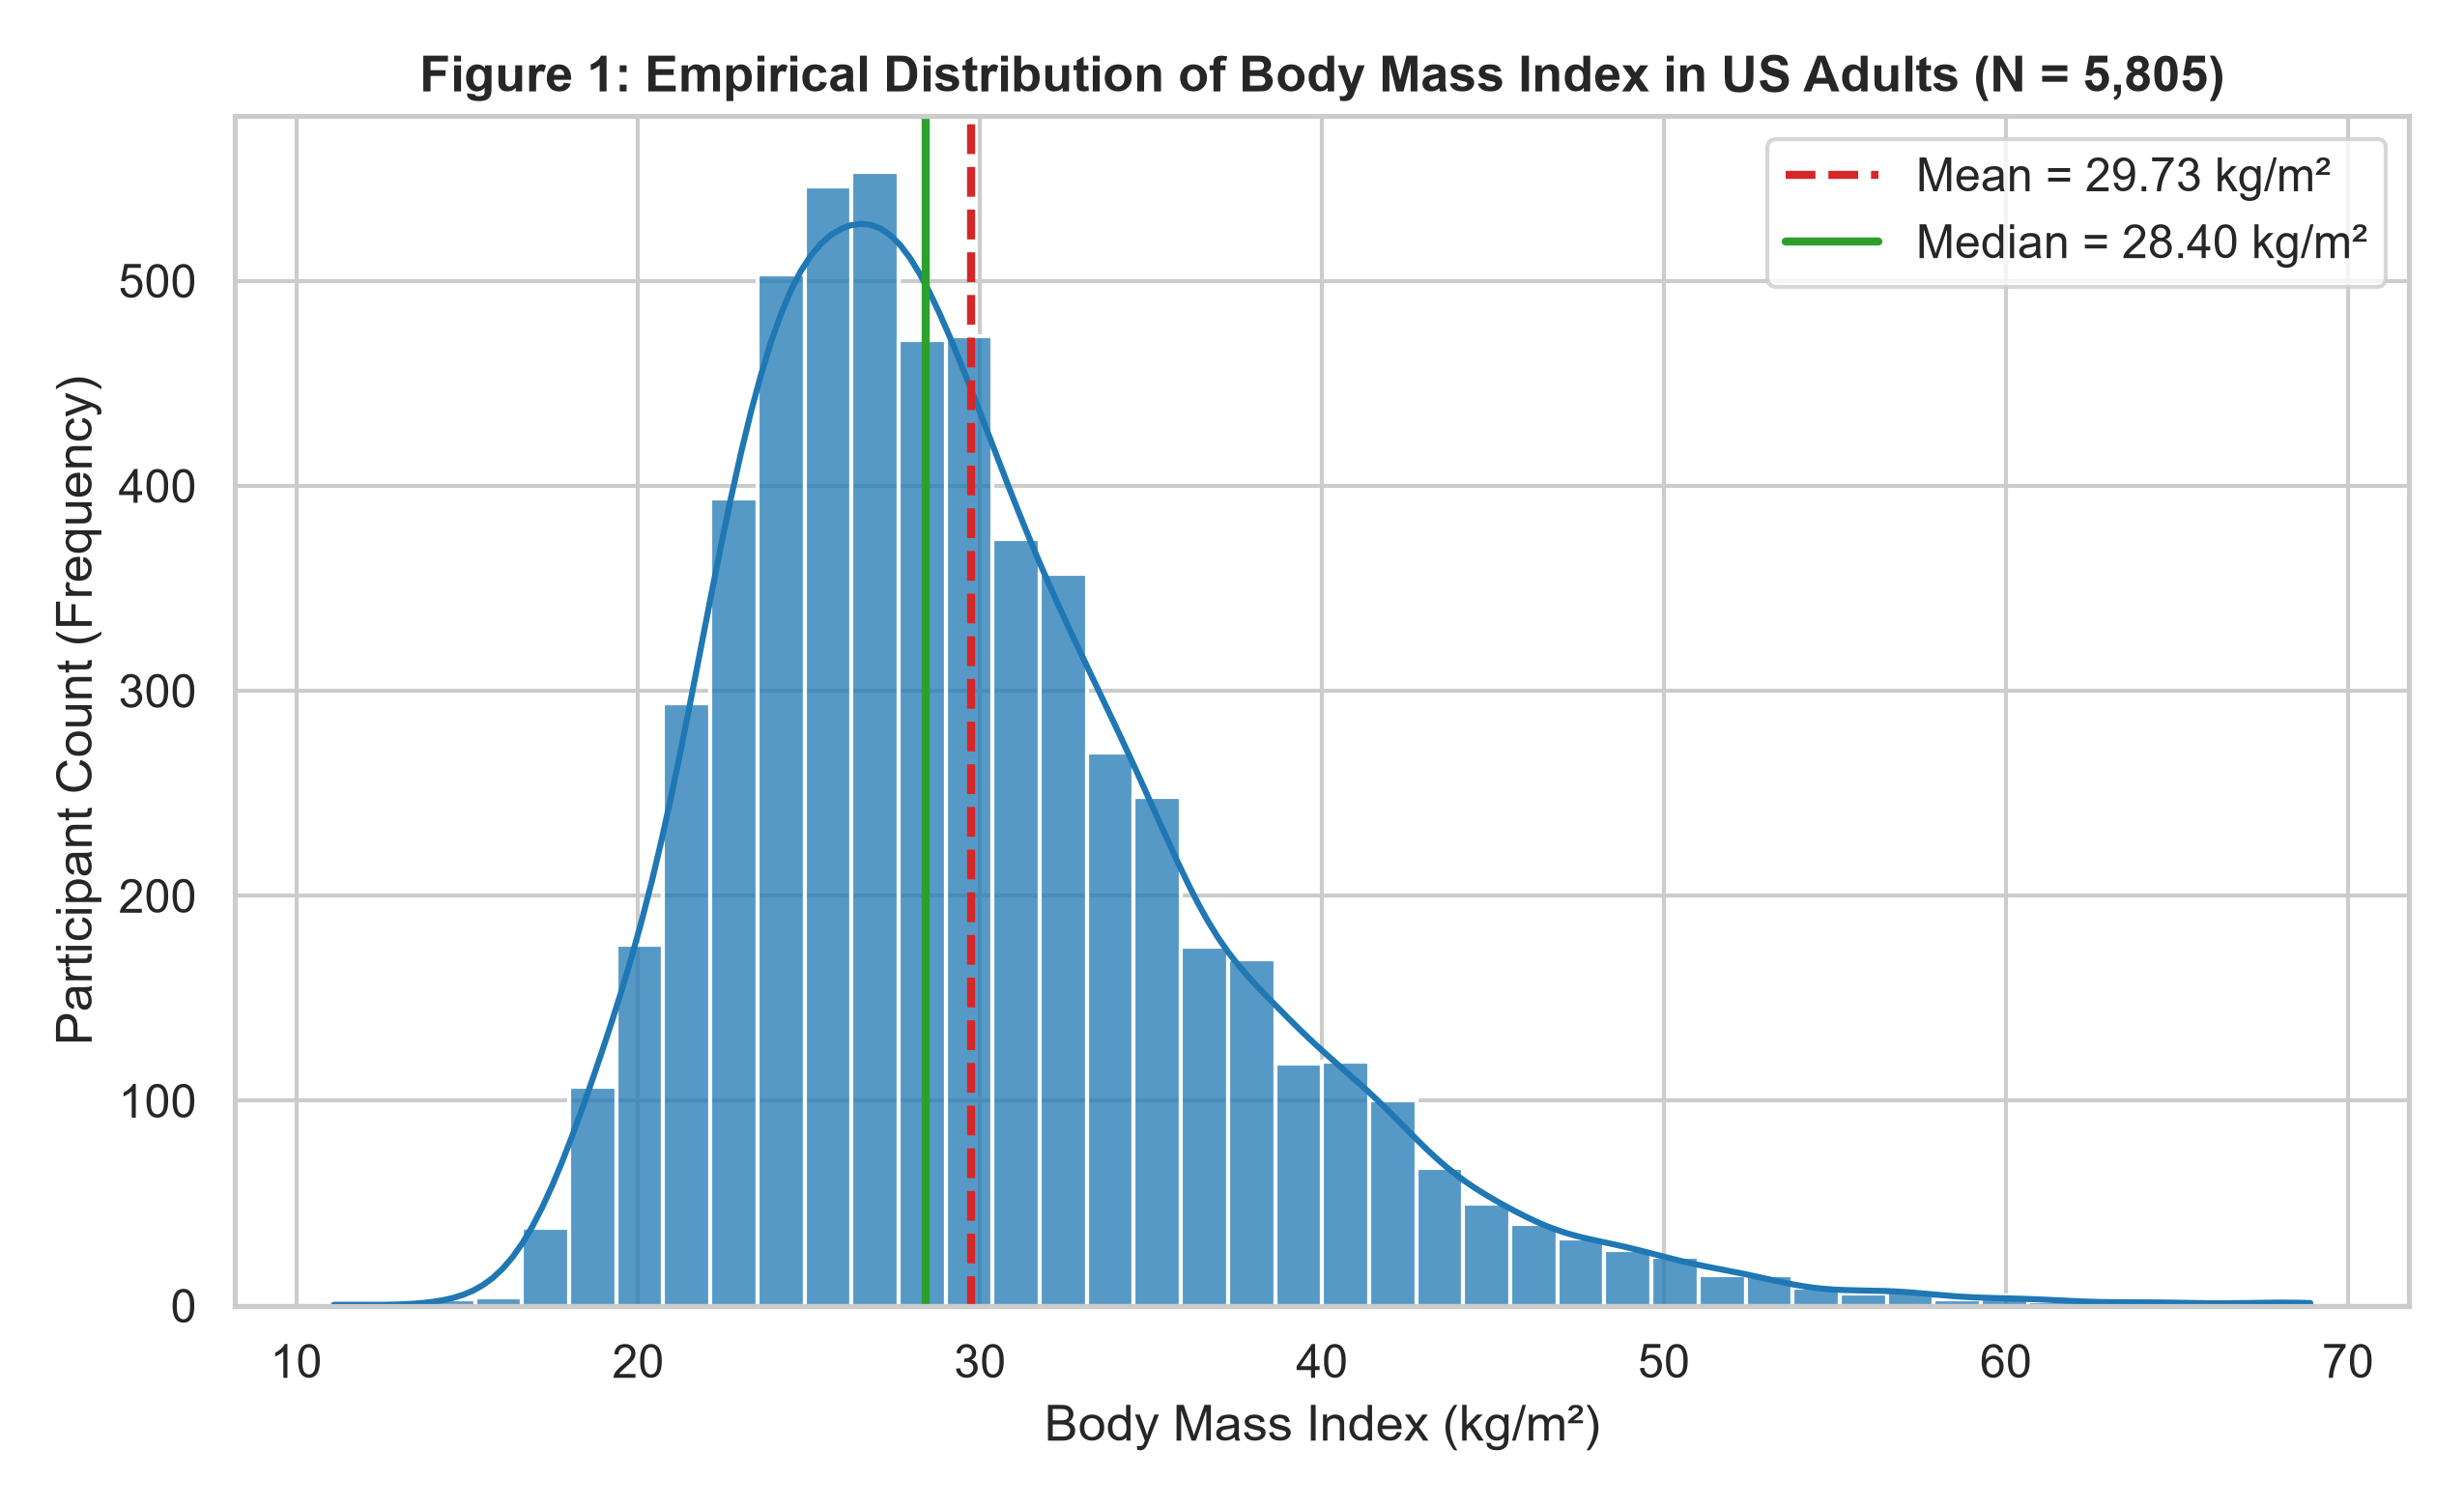
\includegraphics[width=0.84\textwidth]{fig1_bmi_distribution.png}
    \caption{Empirical distribution of Body Mass Index ($\text{kg/m}^2$) in US adults ($N = 5{,}805$), showing kernel density estimate, arithmetic mean ($29.73\text{ kg/m}^2$), and sample median ($28.40\text{ kg/m}^2$).}
    \label{fig:bmi}
\end{figure}

\begin{figure}[H]
    \centering
    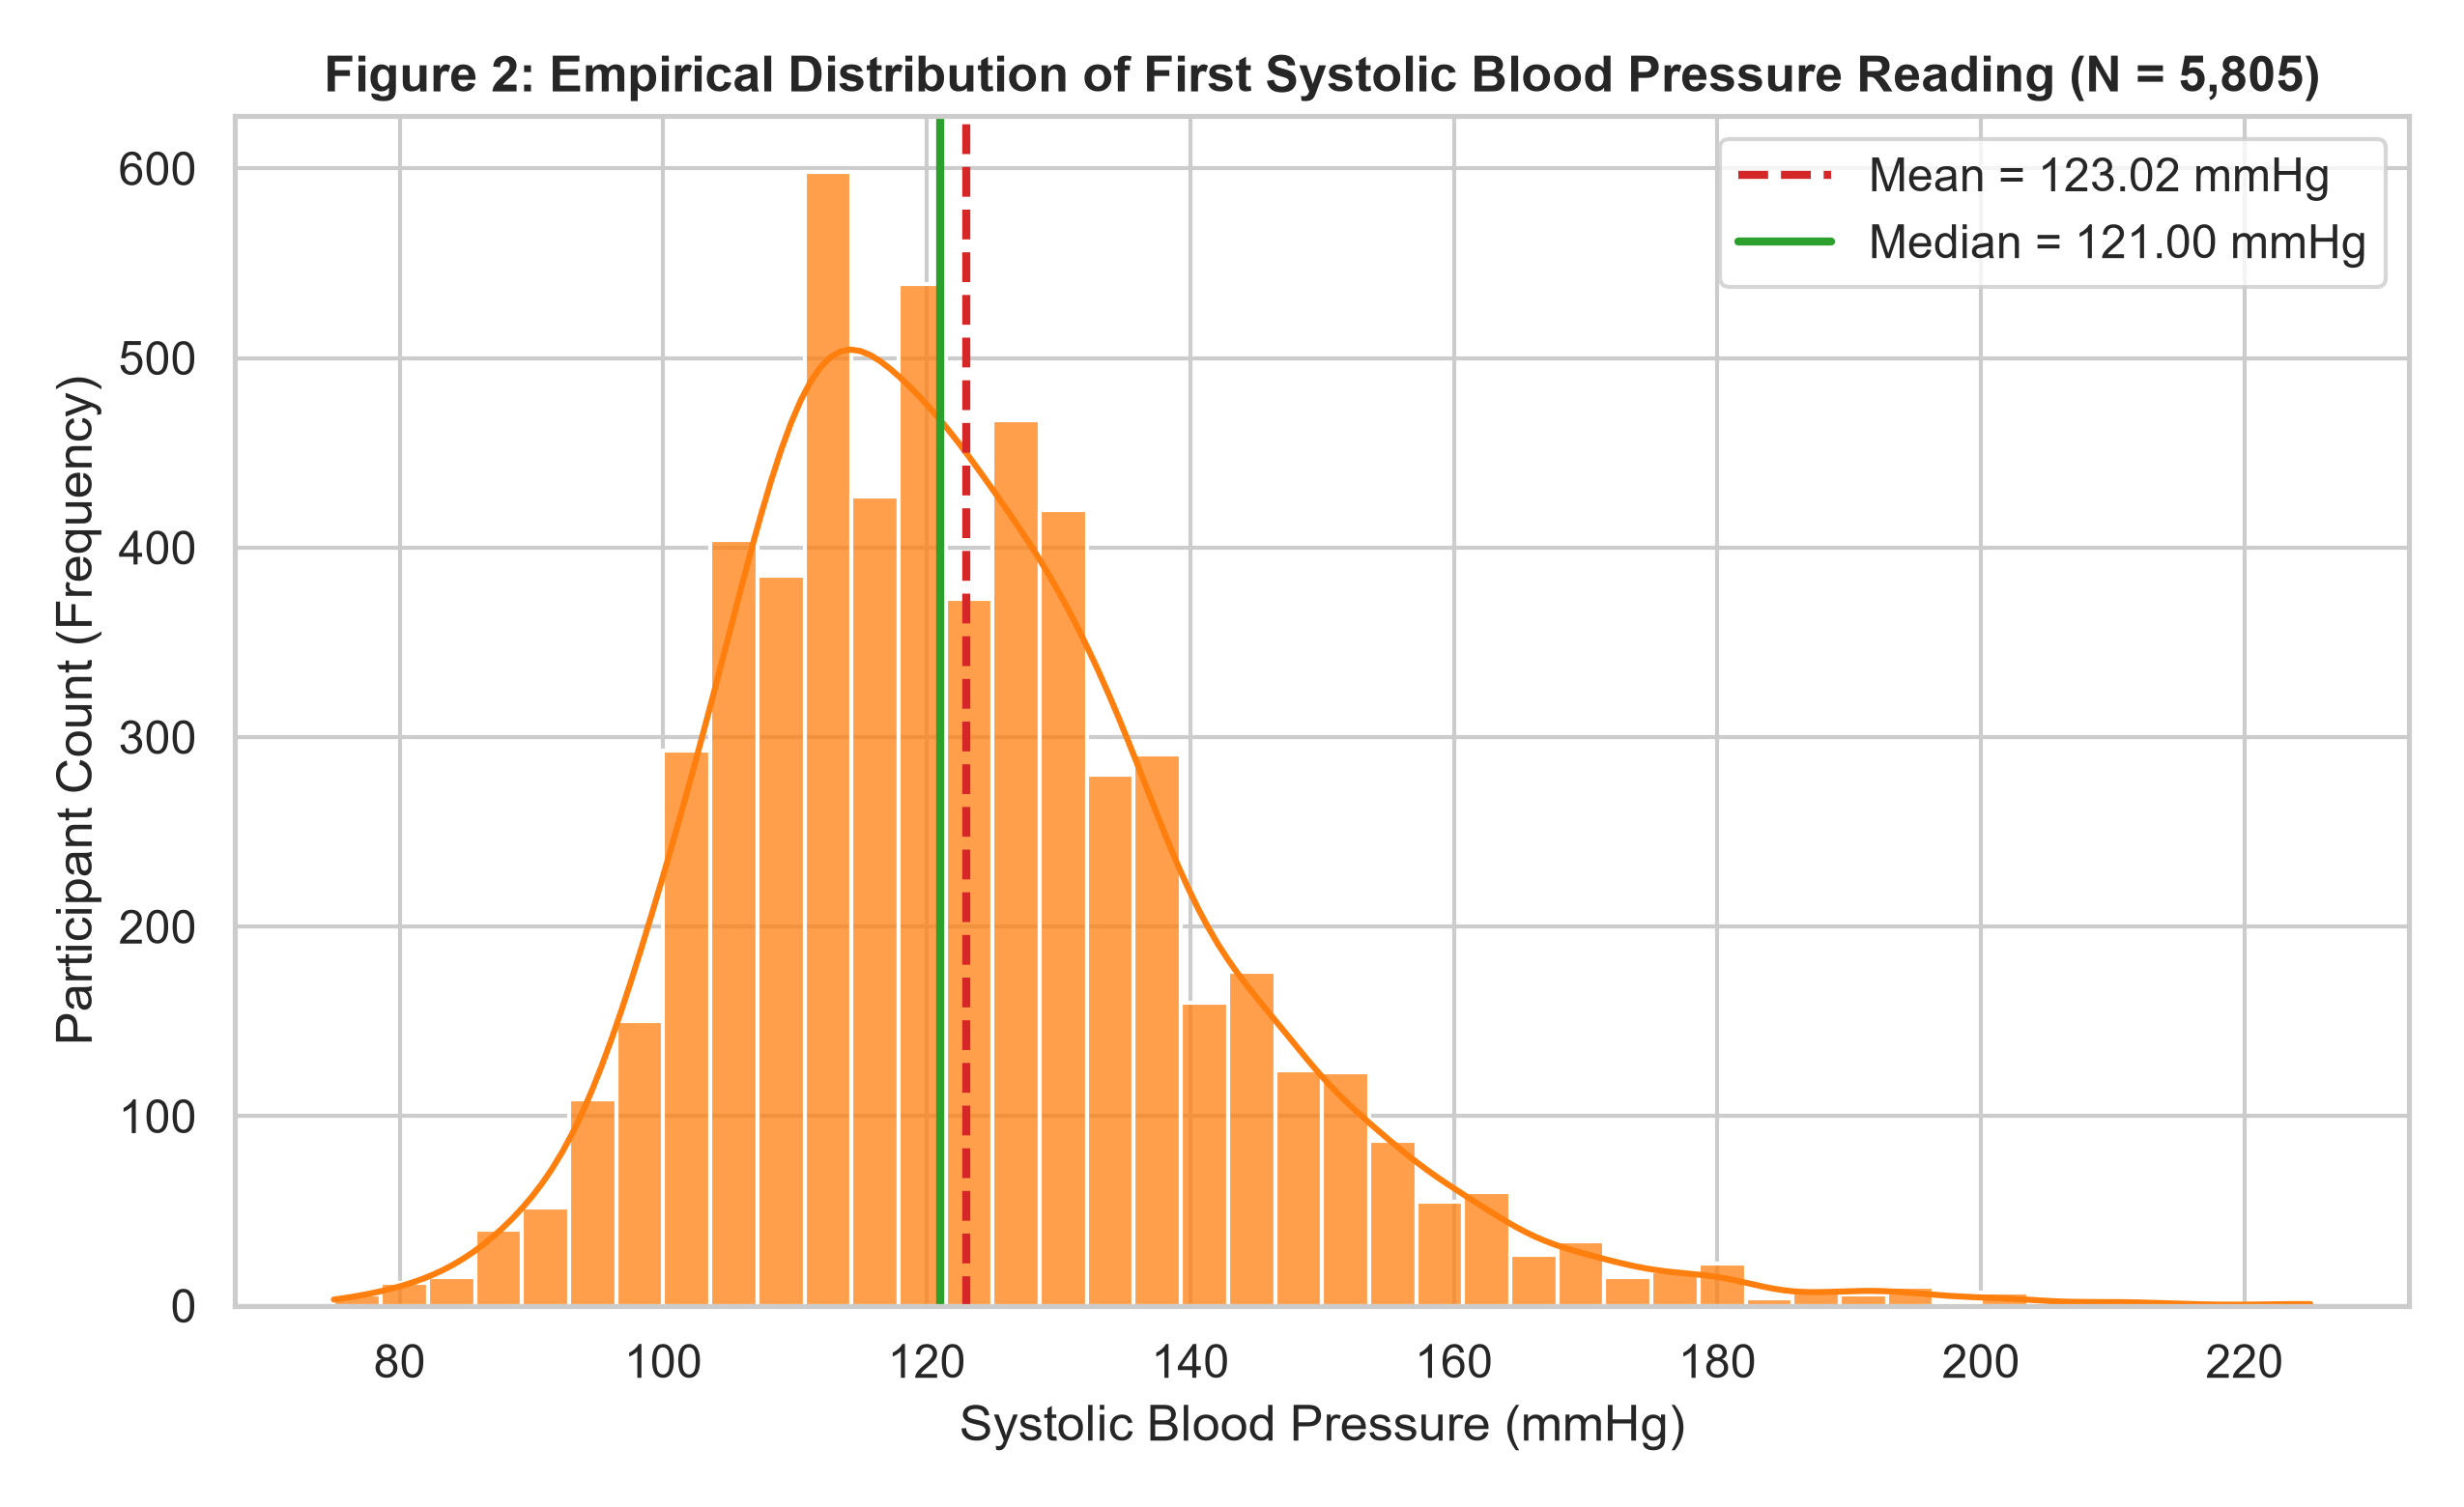
\includegraphics[width=0.84\textwidth]{fig2_sbp_distribution.png}
    \caption{Empirical distribution of first oscillometric Systolic Blood Pressure reading ($\text{mmHg}$) in US adults ($N = 5{,}805$), showing arithmetic mean ($123.02\text{ mmHg}$) and sample median ($121.00\text{ mmHg}$).}
    \label{fig:sbp}
\end{figure}

\begin{figure}[H]
    \centering
    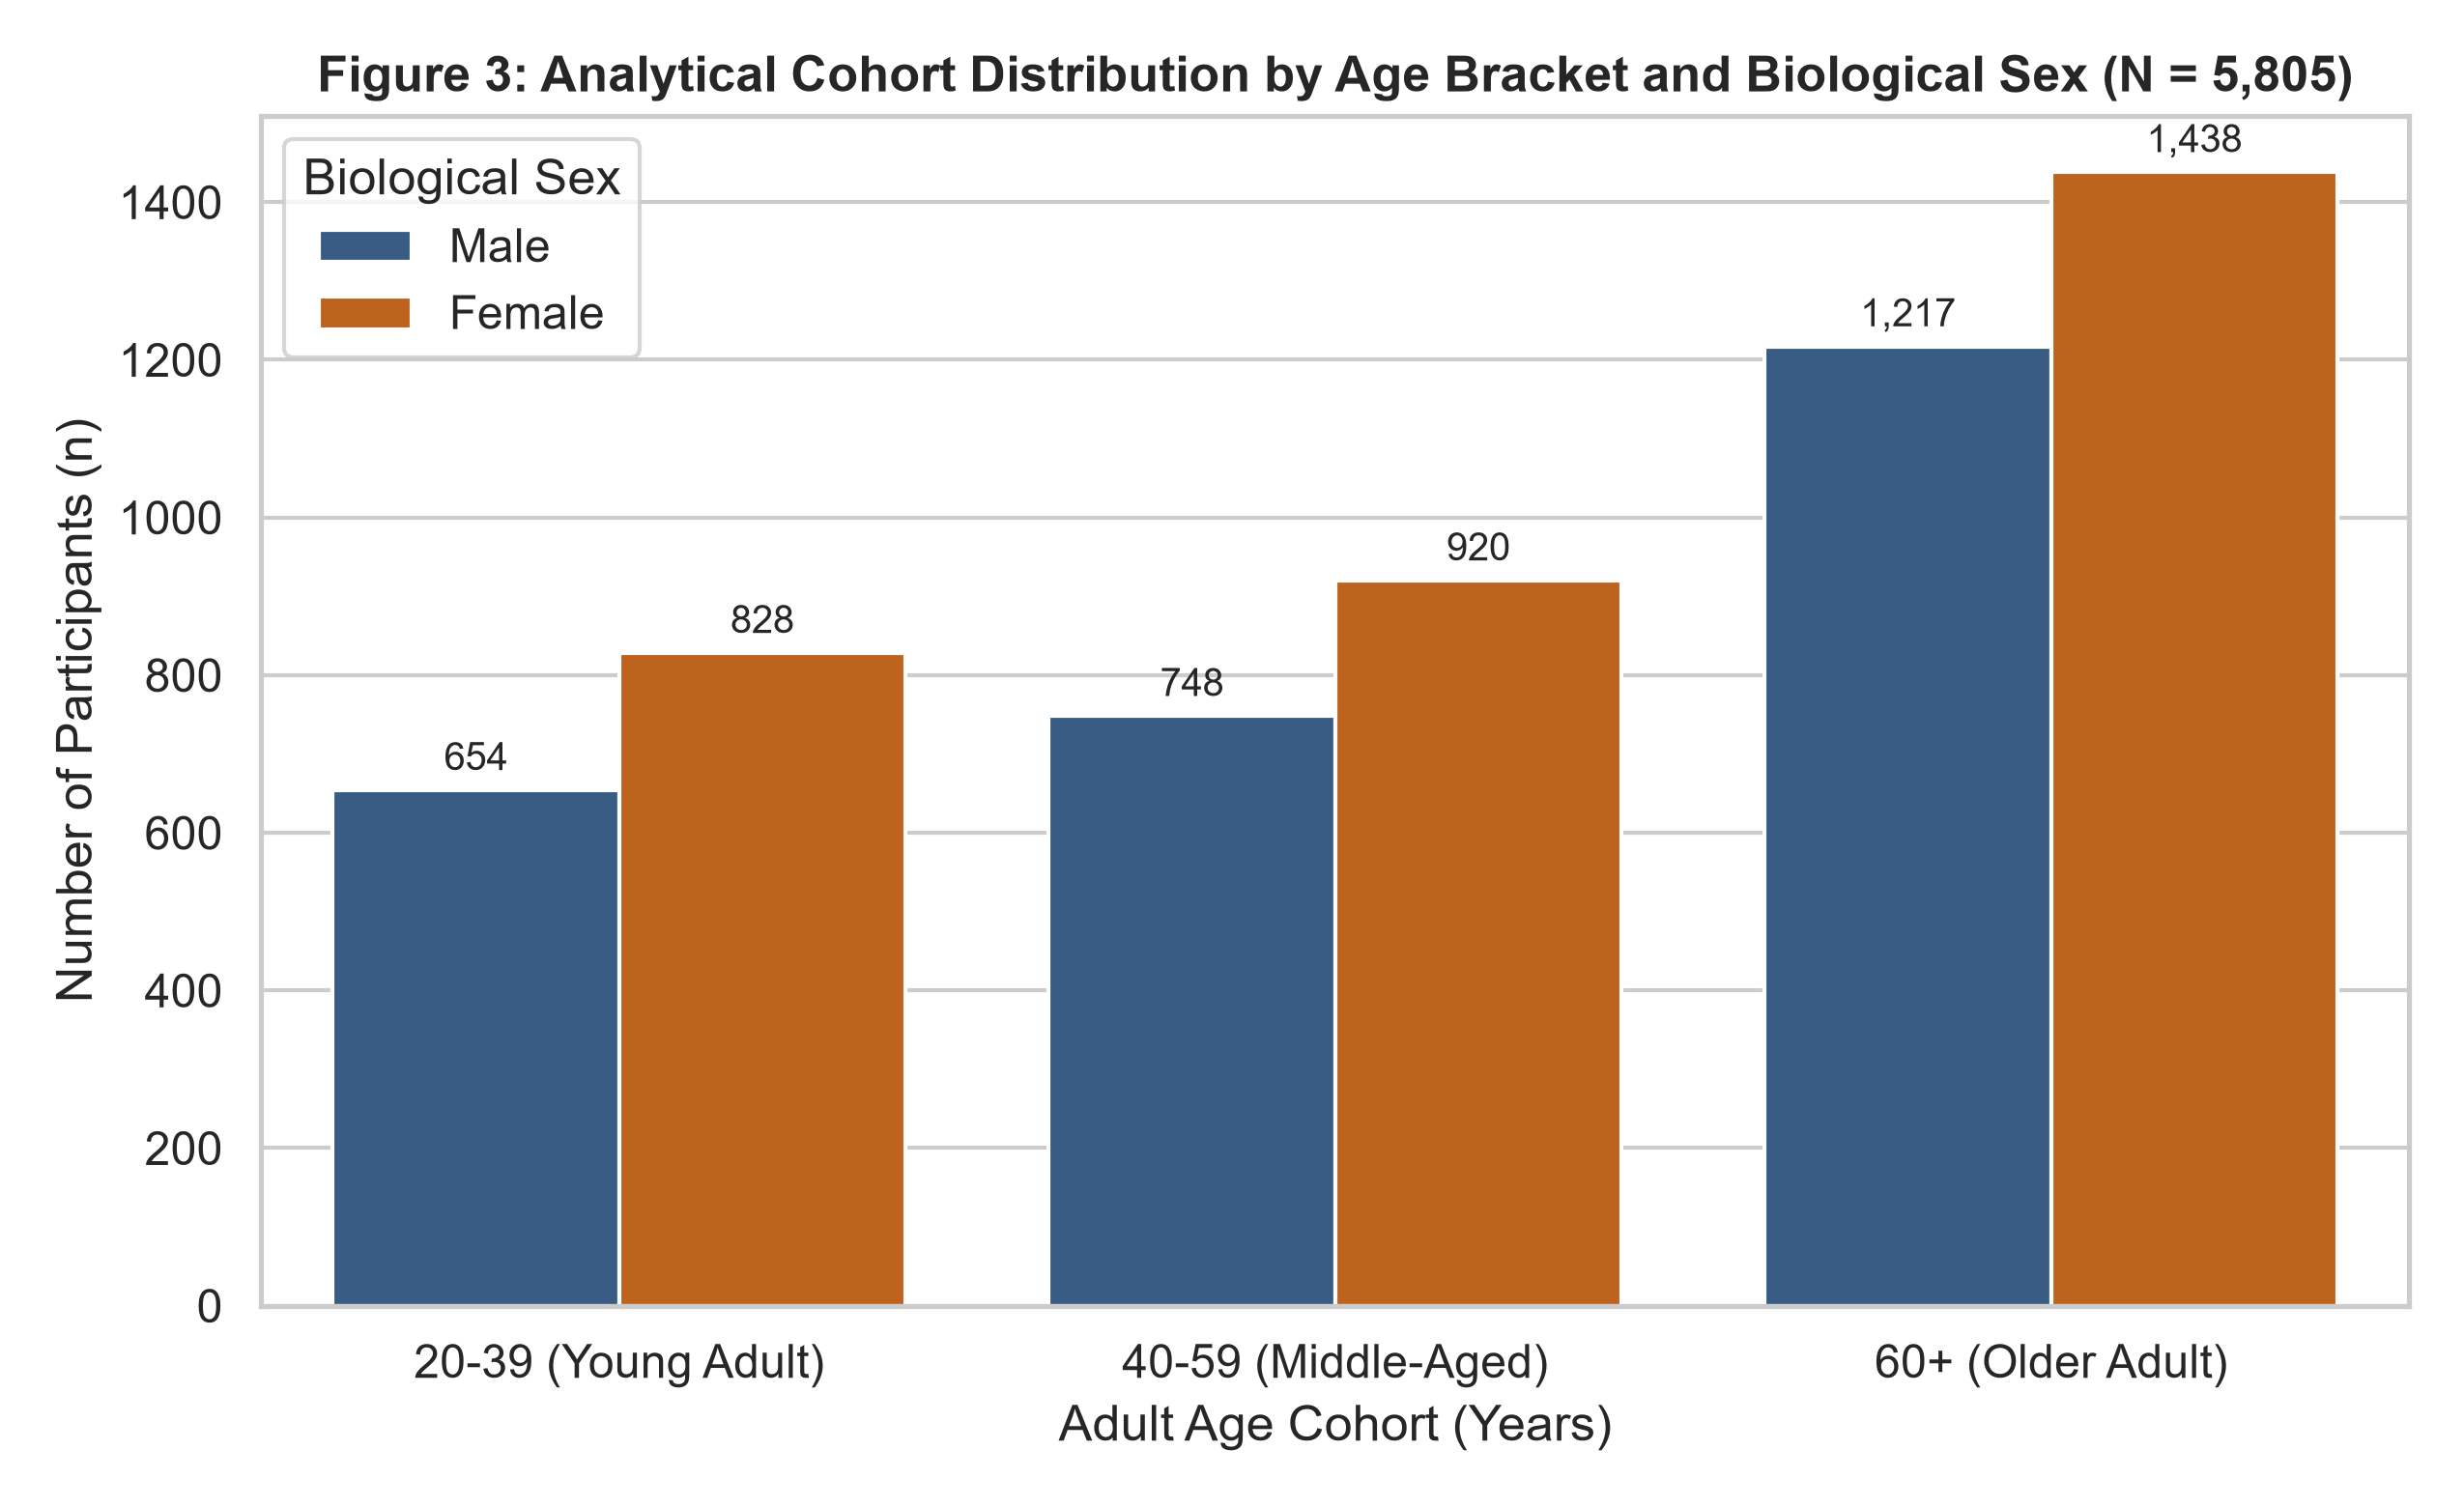
\includegraphics[width=0.84\textwidth]{fig3_demographics.png}
    \caption{Analytical cohort distribution partitioned by adult age bracket and biological sex ($N = 5{,}805$).}
    \label{fig:demographics}
\end{figure}

\begin{figure}[H]
    \centering
    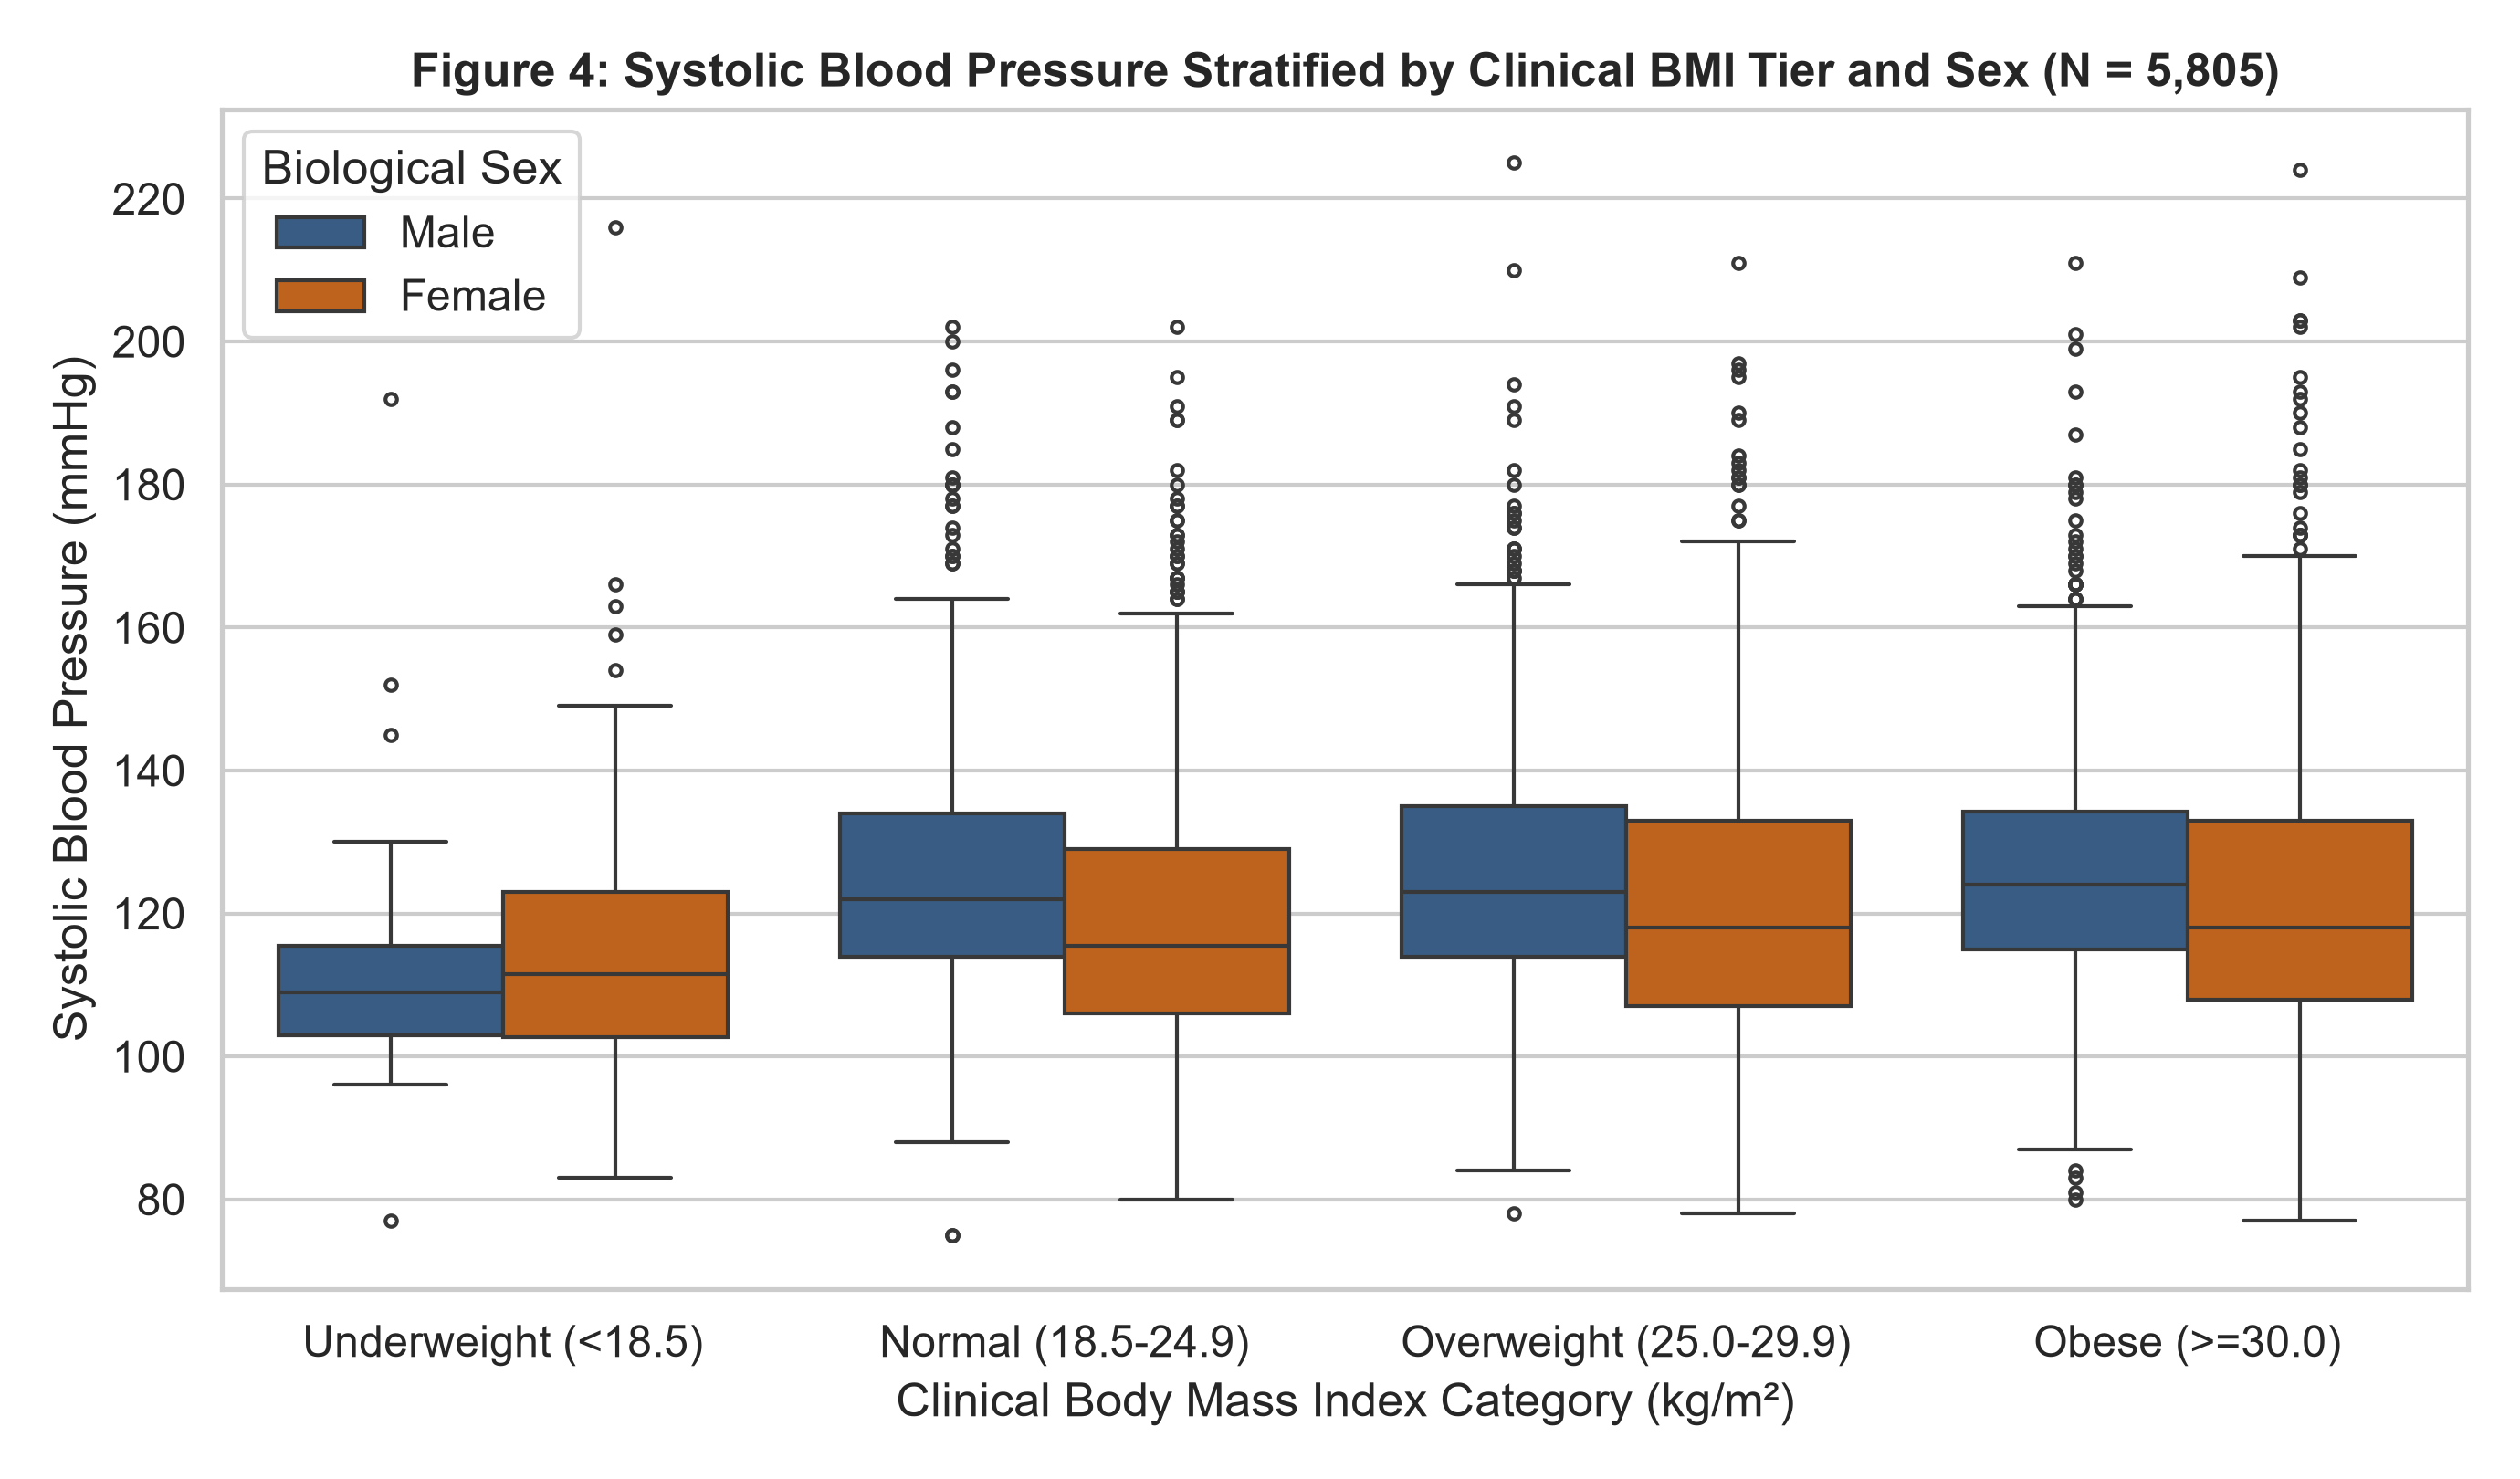
\includegraphics[width=0.88\textwidth]{fig4_bivariate_comparison.png}
    \caption{Stratified boxplots of Systolic Blood Pressure ($\text{mmHg}$) across clinical BMI categories and biological sex ($N = 5{,}805$).}
    \label{fig:bivariate}
\end{figure}

\subsection{Descriptive Bivariate Subgroup Comparisons (Task 9)}
To complement Figure \ref{fig:bivariate} numerically, Table \ref{tab:bivariate_bmi} presents the conditional descriptive summaries of Systolic Blood Pressure (\texttt{BPXOSY1}) partitioned across clinical BMI categories and biological sex, and Table \ref{tab:bivariate_age} presents SBP and BMI partitioned across adult age cohorts and biological sex.

\begin{table}[H]
\centering
\caption{Descriptive Comparison of Systolic Blood Pressure ($\text{mmHg}$) Stratified by BMI Tier and Sex (Task 9)}
\label{tab:bivariate_bmi}
\small
\begin{tabular}{llrrrrrr}
\toprule
\textbf{BMI Category} & \textbf{Sex} & $\mathbf{n}$ & \textbf{Mean} & \textbf{SD} & \textbf{Median} & \textbf{IQR} & \textbf{Weighted Mean} \\
\midrule
Underweight ($< 18.5$)    & Female & 60    & 115.45 & 22.97 & 111.50 & 20.25 & 112.29 \\
                          & Male   & 23    & 114.52 & 22.99 & 109.00 & 12.50 & 111.51 \\
\addlinespace
Normal ($18.5\text{--}24.9$) & Female & 836   & 119.56 & 19.22 & 115.50 & 23.00 & 116.80 \\
                          & Male   & 639   & 125.80 & 18.19 & 122.00 & 20.00 & 123.48 \\
\addlinespace
Overweight ($25.0\text{--}29.9$) & Female & 915 & 121.43 & 19.45 & 118.00 & 26.00 & 119.16 \\
                          & Male   & 957   & 125.39 & 16.99 & 123.00 & 21.00 & 123.02 \\
\addlinespace
Obese ($\ge 30.0$)        & Female & 1,375 & 121.61 & 18.90 & 118.00 & 25.00 & 119.78 \\
                          & Male   & 1,000 & 125.89 & 16.30 & 124.00 & 19.25 & 125.44 \\
\bottomrule
\end{tabular}
\end{table}

\begin{table}[H]
\centering
\caption{Descriptive Comparison of Systolic Blood Pressure ($\text{mmHg}$) and BMI ($\text{kg/m}^2$) Stratified by Age Group and Sex (Task 9)}
\label{tab:bivariate_age}
\small
\setlength{\tabcolsep}{5pt}
\begin{tabular}{llrrrrrrr}
\toprule
\textbf{Age Cohort} & \textbf{Sex} & $\mathbf{n}$ & \textbf{SBP Mean} & \textbf{SBP SD} & \textbf{SBP Med} & \textbf{SBP IQR} & \textbf{SBP Wt Mean} & \textbf{BMI Mean} \\
\midrule
20--39 (Young Adult) & Female & 828   & 108.95 & 11.60 & 108.00 & 13.00 & 108.30 & 29.91 \\
                     & Male   & 654   & 119.08 & 11.49 & 119.00 & 15.00 & 118.63 & 28.63 \\
\addlinespace
40--59 (Middle-Aged) & Female & 920   & 118.62 & 16.78 & 117.00 & 21.00 & 117.91 & 30.81 \\
                     & Male   & 748   & 124.78 & 16.05 & 123.00 & 18.25 & 124.98 & 30.06 \\
\addlinespace
60+ (Older Adult)    & Female & 1,438 & 129.25 & 20.22 & 127.00 & 26.00 & 129.96 & 29.82 \\
                     & Male   & 1,217 & 129.58 & 19.04 & 128.00 & 23.00 & 129.30 & 29.08 \\
\bottomrule
\end{tabular}
\end{table}

\textbf{Non-Inferential Descriptive Synthesis:} Across the $N = 5{,}805$ examined adults, three key descriptive patterns emerge from Tables \ref{tab:bivariate_bmi} and \ref{tab:bivariate_age}:
\begin{enumerate}
    \item \textbf{Adiposity Gradient:} Among males, the unweighted median SBP increases monotonically across all four BMI tiers ($109.00 \to 122.00 \to 123.00 \to 124.00\text{ mmHg}$). Among females, the \texttt{WTMEC2YR}-weighted mean SBP increases monotonically across all tiers ($112.29 \to 116.80 \to 119.16 \to 119.78\text{ mmHg}$), while the female median rises from Underweight ($111.50\text{ mmHg}$) and Normal ($115.50\text{ mmHg}$) to Overweight ($118.00\text{ mmHg}$) and plateaus in the Obese tier ($118.00\text{ mmHg}$).
    \item \textbf{Age Confounding in Marginal BMI Comparisons:} Notice in Table \ref{tab:bivariate_bmi} that for males, the mean SBP in the Normal BMI tier ($125.80\text{ mmHg}$ raw; $123.48\text{ mmHg}$ weighted) is slightly higher than in the Overweight tier ($125.39\text{ mmHg}$ raw; $123.02\text{ mmHg}$ weighted) before rising in the Obese tier ($125.89\text{ mmHg}$ raw; $125.44\text{ mmHg}$ weighted). Table \ref{tab:bivariate_age} reveals the mechanism behind this pattern: older adults (60+ years) have lower mean BMI than middle-aged adults (e.g., $29.08$ vs. $30.06\text{ kg/m}^2$ in males) but substantially higher SBP ($129.58$ vs. $124.78\text{ mmHg}$). Because older men are heavily represented in the Normal and Overweight tiers, age acts as a strong confounding variable when inspecting marginal SBP across BMI categories.
    \item \textbf{Sex Differences and Age-Related Dispersion:} Males exhibit descriptively higher central SBP values than females across the Normal, Overweight, and Obese tiers. Table \ref{tab:bivariate_age} shows that the male-female SBP gap is largest in young adults ($119.08$ vs. $108.95\text{ mmHg}$, a $10.13\text{ mmHg}$ difference) and narrows in middle-aged adults ($124.78$ vs. $118.62\text{ mmHg}$), before nearly converging in the 60+ cohort ($129.58$ vs. $129.25\text{ mmHg}$), while SBP dispersion ($\text{SD}$ and $\text{IQR}$) widens markedly with advancing age in both sexes.
\end{enumerate}

\textit{Methodological Note:} In strict compliance with Phase 1 guidelines, these observations describe empirical sample patterns only; formal hypothesis testing, confidence intervals, and $p$-values are deferred to Phase 3.

% =========================================================================
\section{Refinement of the Statistical Question (Task 10)}
% =========================================================================

Based on our data quality audit, sample size verification ($N = 5{,}805$), and exploratory findings demonstrating the strong confounding role of age, we refine our primary statistical inquiry for Phases 2 through 5 as follows:

\begin{quote}
\textbf{Refined Statistical Question:} \textit{``Among civilian, non-institutionalized United States adults aged 20 years and older in NHANES 2021--2023 ($N = 5{,}805$), how strongly is Body Mass Index (\texttt{BMXBMI}) associated with first oscillometric Systolic Blood Pressure (\texttt{BPXOSY1}) after accounting for age (\texttt{RIDAGEYR}) and biological sex (\texttt{RIAGENDR}), and how do complex survey sampling weights (\texttt{WTMEC2YR}) modify probability, interval estimation, and linear regression conclusions?''}
\end{quote}

\textbf{Suitability of the Analytical Dataset:}
\begin{enumerate}
    \item \textbf{Statistical Power and Sample Size:} With $N = 5{,}805$ complete adult observations and substantial representation across all sex, age, and BMI strata, the dataset supports stable conditional probability estimation (Phase 2), parametric and bootstrap confidence intervals and ANOVA (Phase 3), and multiple ordinary least squares and weighted least squares regression (Phases 4 and 5).
    \item \textbf{Measurement Precision:} Both primary continuous variables (\texttt{BMXBMI} and \texttt{BPXOSY1}) are objectively measured by trained clinical staff in the MEC rather than self-reported, minimizing recall bias.
    \item \textbf{Traceable Reproducibility:} Every filtering step from raw CDC SAS transport files to final summary tables and figures is fully automated in \texttt{src/download\_data.py} and \texttt{src/phase1\_analysis.py}.
\end{enumerate}

\end{document}